\documentclass{beamer}
\usepackage[T1]{fontenc}
\usepackage[utf8]{inputenc}
\usepackage[german]{babel}
\usepackage{pdfpages}
\usepackage{amssymb}
\usepackage{enumerate}
\usepackage{array}
\usepackage{lmodern}
\usepackage{url}
\usepackage{hyperref}
\usepackage[all]{xy}
\usepackage[export]{adjustbox}
\usepackage{subcaption}
\usepackage{listings}
\usepackage{tikz}
\usetikzlibrary{arrows,positioning,fit,shapes,calc}

\usepackage{graphicx}
\graphicspath{{./img/}}

\usepackage{enumitem}
\newlist{todolist}{itemize}{2}
\setlist[todolist]{label=$\square$}
\usepackage{pifont}
\newcommand{\cmark}{\ding{51}}%
\newcommand{\xmark}{\ding{55}}%
\newcommand{\done}{\rlap{$\square$}{\raisebox{1pt}{\large\hspace{1pt}\cmark}}%
\hspace{-1pt}}
\newcommand{\wontfix}{\rlap{$\square$}{\raisebox{1.5pt}{\large\hspace{.5pt}\xmark}}
\hspace{-2.5pt}}

%Farbschema
\definecolor{tuerkis}{rgb}{0.0, 0.65, 0.76}
\definecolor{weiss}{rgb}{1.0,1.0,1.0}
\definecolor{gruen}{rgb}{0.22, 0.74, 0.07}

\usetheme{metropolis}
\setbeamercolor{progress bar}{fg=gruen,bg=gruen}
\setbeamercolor{frametitle}{fg=black, bg = gruen}
\setbeamercolor{background canvas}{bg = weiss}
\setbeamercolor{footline}{fg=gray}
\setbeamerfont{page number in head/foot}{size=\scriptsize}
\setbeamercolor{title}{fg = black}
\setbeamertemplate{frame footer}{ \insertlogo{\includegraphics[width=0.1\textwidth]{aegis_logo_with_name.pdf}}\hfill\insertsection}

\lstset{frame=single}

\title{SWP 21 - Gruppe 01: Abwehr von Denial-of-Service-Angriffen durch effiziente User-Space Paketverarbeitung} 
\subtitle{Abschlussveranstaltung}
\institute{Technische Universität Ilmenau}
\date{21. Juli 2021}

\begin{document}

\begin{frame}
    \maketitle
\end{frame}

\begin{frame}{Das Problem DDoS\footnotemark}
    \center
    \begin{itemize}
        \pause
        \item \alert{Einfach} und \alert{beliebt}
              \pause
        \item Fast \alert{unaufhaltsam}
              \pause
        \item Abwehr komplex und \alert{ressourcenintensiv}
              \pause
        \item Angriffsvolumen \alert{verdoppelt} mindestens jährlich  \footnotemark
              \pause
        \item Schäden bei $\sim$323.400 Euro je Stunde \footnotemark
    \end{itemize}

    \only<5->{\footnotetext[1]{ns-cdn.neustar.biz}}
    \only<6->{\footnotetext[2]{https://it-service.network}}
    \footnotetext[3]{DDoS = Distributed Denial of Service}
\end{frame}

{
%\setbeamercolor{background canvas}{bg=black}
\usebackgroundtemplate{\includegraphics[width=\paperwidth,height=\paperheight]{Hintergrund.pdf}}
\begin{frame}[plain]
    \begin{center}
        \color{green}{Abwehr von Denial-of-Service-Angriffen

            durch effiziente User-Space Paketverarbeitung}

        \vspace{\baselineskip}\pause
        \includegraphics[width=.8\linewidth]{aegis_logo_with_name.pdf}
    \end{center}
\end{frame}
}

\begin{frame}{Wie funktioniert AEGIS?}
    \only<1>{
        \begin{center}
            \includegraphics[width=\linewidth]{Netzwerkplan-Real.png}
        \end{center}
    }
    \only<2>{
        \begin{center}
            \begin{tikzpicture}[node distance=1cm, on grid,
                    every actor role/.style = {},
                    actor role/.style = {rectangle, draw=black!80, ultra thick, minimum size = 6mm, every actor role},
                    composite actor role/.style = {fill=blue!20, actor role},
                    elementary actor role/.style = {fill=white!100, actor role}]
                % external left
                \node at (0,0) [cloud, draw =blue, text=black, fill = gray!10, aspect=1.5, cloud puffs = 18, cloud puff arc = 90, font=\small] (external) {Internet};
                % internal right
                \node at (8,0) [composite actor role] (internal) [minimum height=24mm, text width=17mm, align=center] {internes  Netzwerk};
                %connection
                \draw[xshift=1cm,draw=black] (external) -- (internal);
            \end{tikzpicture}
        \end{center}
    }
    \only<3>{
        \begin{center}
            \begin{tikzpicture}[node distance=1cm, on grid,
                    every transaction/.style = {fill=white!100},
                    transaction/.style = {diamond, draw, every transaction, font=\small},
                    every actor role/.style = {},
                    actor role/.style = {rectangle, draw=black!80, ultra thick, minimum size = 6mm, every actor role},
                    composite actor role/.style = {fill=blue!20, actor role},
                    elementary actor role/.style = {fill=white!100, actor role},
                    initiator/.style = {-},
                    executor/.style = {<-, >=},
                    system/.style = {rectangle, fill=white!100, ultra thick, draw=black!80,
                            minimum height=23mm, minimum width=3.8cm} ]

                \node [system] (system) at (0,3){};
                \node [above, text width=2cm, align=center] at (system.north) {AEGIS};
                \node [transaction] (nic1) at($(system.south west)!.50!(system.north west)$) {NIC\_1};
                \node [transaction] (nic2) at($(system.south east)!.50!(system.north east)$) {NIC\_2};

                % external left
                \path (nic1)++(-2.5,0) node [cloud, draw =blue, text=black, fill = gray!10, aspect=1.5, cloud puffs = 18, cloud puff arc = 90, font=\small] (external) {Internet} edge  [executor] (nic1);
                % internal right
                \path (nic2)++(2.5,0) node [composite actor role] (internal) [minimum height=24mm, text width=17mm, align=center] {internes  Netzwerk} edge  [executor] (nic2);

            \end{tikzpicture}
        \end{center}
    }
    \only<4>{
        \begin{center}
            \begin{tikzpicture}[node distance=1cm, on grid,
                    every transaction/.style = {fill=white!100},
                    transaction/.style = {diamond, draw, every transaction, font=\small},
                    every actor role/.style = {},
                    actor role/.style = {rectangle, draw=black!80, ultra thick, minimum size = 6mm, every actor role},
                    composite actor role/.style = {fill=blue!20, actor role},
                    elementary actor role/.style = {fill=white!100, actor role},
                    initiator/.style = {-},
                    executor/.style = {<-, >=},
                    system/.style = {rectangle, fill=white!100, ultra thick, draw=black!80,
                            minimum height=60mm, minimum width=3.8cm} ]

                \node [system] (system) at (0,3){};
                \node [above, text width=2cm, align=center] at (system.north) {AEGIS};
                \node [transaction] (nic1) at($(system.south west)!.80!(system.north west)$) {NIC\_1};
                \node [transaction] (nic2) at($(system.south east)!.180!(system.north east)$) {NIC\_2};

                \draw[xshift=1cm,draw=black] (nic1) -- ($(nic1)+(1.5,0)$) -- ($(nic2)-(2.4,0)$) --(nic2);
                \draw[xshift=1cm,draw=black] (nic1) -- ($(nic1)+(1.7,0)$) -- ($(nic2)-(2.2,0)$) --(nic2);
                \draw[xshift=1cm,draw=black] (nic1) -- ($(nic1)+(2.2,0)$) -- ($(nic2)-(1.7,0)$) --(nic2);
                \draw[xshift=1cm,draw=black] (nic1) -- ($(nic1)+(2.4,0)$) -- ($(nic2)-(1.5,0)$) --(nic2);

                \node [composite actor role] (PacketDissection) at ($(system.south)!.60!(system.north)$) {PacketDissection};
                \node [composite actor role] (Inspection) at ($(system.south)!.45!(system.north)$) {Inspection} edge [executor] (PacketDissection);
                \node [composite actor role] (Treatment) at ($(system.south)!.30!(system.north)$) {Treatment} edge [executor] (Inspection);
                \node [composite actor role] (Statistic) at ($(system.south)!.10!(system.north)$) {Statistic} edge [executor] (Treatment);

                \draw[xshift=1cm,draw=black] (nic1) -- ($(system.south)!.80!(system.north)$) -- (PacketDissection);
                \draw[xshift=1cm,draw=black] (Treatment) -- ($(system.south)!.18!(system.north)$) -- (nic2);

                % external left
                \path (nic1)++(-2.5,0) node [cloud, draw=blue, text=black, fill = gray!10, aspect=1.5, cloud puffs = 18, cloud puff arc = 90, font=\small] (external) {Internet} edge  [executor] (nic1);
                % internal right
                \path (nic2)++(2.5,0) node [composite actor role] (internal) [minimum height=24mm,text width=17mm, align=center] {internes  Netzwerk} edge  [executor] (nic2);
            \end{tikzpicture}
        \end{center}
    }
\end{frame}

\begin{frame}{Was kann AEGIS?}

    \center
    \begin{todolist}
        \only<1>{\item Abwehr von SYN Flood Attacken}
        \only<2->{\item[\done] Abwehr von SYN Flood Attacken}
        \only<1-2>{\item Abwehr von SYN-FIN/SYN-FIN-ACK Attacken}
        \only<3->{\item[\done] Abwehr von SYN-FIN/SYN-FIN-ACK Attacken}
        \only<1-3>{\item Datenrate $\geq$ 5 Gbit/s \footnote{Gigabit per second}; Paketrate $\geq$ 7 Mpps \footnote{Million packages per second}}
        \only<4->{\item[\done] Datenrate $\geq$ 5 Gbit/s \footnote{Gigabit per second}; Paketrate $\geq$ 7 Mpps \footnote{Million packages per second}}
        \only<1-4>{\item Konfiguration durch Nutzer}
        \only<5->{\item[\done] Konfiguration durch Nutzer}
        \only<1-5>{\item Skalieren}
        \only<6->{\item[\done] Skalieren}
    \end{todolist}
\end{frame}

\begin{frame}{Was kostet AEGIS?}
    \begin{todolist}
        \item Leistungsfähiger Rechner mit Multicore CPU \pause
        \item DPDK-fähige Netzwerkkarte \pause
        \item Stromkosten von $\sim$1000€ p.a. \pause
        \item Delay für Verbindungen aus dem internen Netz: 0\% \pause
        \item Delay für Verbindungen aus dem externen Netz: $<30$\%
    \end{todolist}
\end{frame}

\begin{frame}{Der Testaufbau}
    \begin{center}
        \begin{tikzpicture}[node distance=1cm, on grid,
                every transaction/.style = {fill=white!100},
                transaction/.style = {diamond, draw, every transaction, font=\small},
                every actor role/.style = {},
                actor role/.style = {rectangle, draw=black!80, ultra thick, minimum size = 6mm, every actor role},
                composite actor role/.style = {fill=blue!20, actor role},
                elementary actor role/.style = {fill=white!100, actor role},
                initiator/.style = {-},
                executor/.style = {<-, >=},
                system/.style = {rectangle, fill=blue!20, ultra thick, draw=black!80,
                        minimum height=10mm, minimum width=20mm} ]
            \node [system] (system) at (0,3){Dave};
            \node [above, text width=2cm, align=center] at (system.north) {AEGIS};
            \node [transaction] (nic1) at($(system.south west)!.50!(system.north west)$) {};
            \node [transaction] (nic2) at($(system.south east)!.50!(system.north east)$) {};
            \path (nic1)++(-2.5,+2) node [composite actor role] (mallory)[minimum height=4mm] {Mallory} edge  [executor] (nic1);
            \path (nic1)++(-2.5,-2) node [composite actor role] (alice)[minimum height=4mm] {Alice} edge  [executor] (nic1);
            \path (nic2)++( 2.5,0) node [composite actor role] (bob)[minimum height=4mm] {Bob} edge  [executor] (nic2);

            \path[xshift=1cm] (alice) -- node [midway,above,align=center, text width=20mm,rotate=40]{Legitime Verbindung} (nic1);
            \path[xshift=1cm] (mallory) -- node [midway,above,align=center, text width=20mm,rotate=-40]{DoS Attack} (nic1);

            \node [left, text width=.3cm, align=center] at (mallory.west) {\includegraphics[width=10px]{1F608.pdf}};
            \node [left, text width=.3cm, align=center] at (alice.west) {\includegraphics[width=10px]{1F607.pdf}};

        \end{tikzpicture}
    \end{center}
\end{frame}

\begin{frame}{Herausforderungen}
    \center
    \begin{todolist}
        \item Isolation vom Internet durch Network-Namespaces \pause
        \item Nachbau der DPDK-Library für Unit-Tests \pause
        \item Begrenzte Hardwareressourcen des Testbeds \pause
        \item Codeeffizienz als maßgebliches Erfolgskriterium \pause
        \item Notwendigkeit der Entwicklung eigener Angriffstools
    \end{todolist}
\end{frame}

\begin{frame}{Der Angreifer}
    \includegraphics[width=\linewidth]{attackerVShping.pdf}
\end{frame}

\begin{frame}[plain]
    \center
    Live aus dem Labor
\end{frame}

\begin{frame}{Bewertung des Softwareprojekts}
    Aus Umfragen ergab sich:
    \begin{itemize} \pause
        \item \includegraphics[width=8px]{1F600.pdf} Praxiserfahrung \pause
        \item \includegraphics[width=8px]{1F600.pdf} Teamarbeit \pause
        \item \includegraphics[width=8px]{1F600.pdf} Team Programming \pause
        \item \includegraphics[width=8px]{1F635.pdf} Bewältigung komplexer Aufgabenstellungen \pause
        \item \includegraphics[width=8px]{1F600.pdf} Erfahrungen mit Git, \LaTeX, Linux und DPDK \pause
        \item \includegraphics[width=8px]{1F60E.pdf} Ambitionen zur Projektfortführung
    \end{itemize}
\end{frame}

\begin{frame}{Projekt Zeitrahmen}
    \includegraphics[width=\linewidth]{AufwandsschaetzungNeu.pdf}
\end{frame}

\begin{frame}{Zukunftsvisionen}
    \begin{todolist} \pause
        \item Repository auf Github \pause
        \item Erweiterung der Abwehrmechanismen \pause
        \item Statistik für Nutzer \pause
        \item Effizienzsteigerung
    \end{todolist}
\end{frame}

\section{Raum für Fragen}

\end{document}